\documentclass[12pt]{article}
\usepackage[margin=1in]{geometry}
\usepackage{amsmath,amssymb,amsthm,booktabs,graphicx,natbib,microtype}
\newtheorem{theorem}{Theorem}
\newtheorem{proposition}[theorem]{Proposition}
\newtheorem{corollary}[theorem]{Corollary}
\newtheorem{remark}[theorem]{Remark}
\title{Native Spectral-Reset Memory Pairs\\\large A Universal Tail-Mass Theorem and 130 Subunit Loewner Certificates}
\author{Prime Dynamics Theory Program}
\date{July 2026}

\begin{document}
\maketitle

\begin{abstract}
RH-153 proved that a correlated Gram--tail pair transports through reset
overlaps without changing its generalized tail ratio, and RH-154 isolated a
well-conditioned terminal half.  The missing object was a native pair on the
spectral reset packet itself.

Let a geometric memory be $M_t=R_t+T_t$, where $R_t$ contains ages below a
fixed depth $d$ and $T_t$ contains the older terms.  Each normalized snapshot
is positive semidefinite with trace one, so
\[
 \|T_t\|\leq\tau_t:=\sum_{a=d}^{t}\eta^a
 \leq\frac{\eta^d}{1-\eta}.
\]
If $U_t$ is the rank-$r$ top spectral packet of $M_t$ and
$\lambda_r(M_t)\geq\ell_t>\tau_t$, then for the native compressions
$G_t=U_t^*R_tU_t$ and $D_t=U_t^*T_tU_t$ we prove the sharp bound
\[
 D_t\preceq\frac{\tau_t}{\ell_t-\tau_t}G_t.
\]
The ratio is subunit exactly at the scalar-information gate
$\ell_t>2\tau_t$.

Combining the dynamics-free tail mass with the RH-151 outward selected
eigenvalue lowers certifies all 130 frozen snapshots.  The worst ratio upper
is $0.224696$ and the minimum $\ell_t/(2\tau_t)$ margin is $2.72523$.
All 62 RH-154 terminal-half snapshots also certify.  Direct nominal ratios
are much smaller---at most $2.879\times10^{-5}$---but are not needed for the
proof.  This closes a native reset memory pair.  It does not yet identify
that pair with the directional cross-action Gram used in the earlier support
architecture.
\end{abstract}

\section{A reset pair that respects the memory construction}
Let $S_j\succeq0$ with $\operatorname{tr}S_j=1$ and fix
$0\leq\eta<1$.  At time $t$ define
\[
 M_t=\sum_{a=0}^{t}\eta^aS_{t-a},\quad
 R_t=\sum_{0\leq a<d}\eta^aS_{t-a},\quad
 T_t=\sum_{d\leq a\leq t}\eta^aS_{t-a}.
\]
Empty sums are zero.  Then $M_t=R_t+T_t$ exactly.  Unlike an arbitrary
ambient recent Gram, $R_t$ may be singular.  Positivity is recovered only
after compressing to a packet selected by the full memory.

\section{Universal tail mass and packet recovery}
\begin{theorem}[Geometric tail-mass bound]\label{thm:mass}
For every snapshot sequence,
\[
 0\preceq T_t\preceq\tau_t I,
 \qquad
 \tau_t=\sum_{a=d}^{t}\eta^a
 \leq\tau_\infty:=\frac{\eta^d}{1-\eta}.
\]
The constants are sharp from trace-one positivity alone.
\end{theorem}
\begin{proof}
Every eigenvalue of a positive trace-one matrix lies in $[0,1]$, so
$S_j\preceq I$.  Sum the weighted inequalities.  Rank-one snapshots aligned
with one fixed direction attain the operator upper.
\end{proof}

Let $U$ have orthonormal columns spanning the top $r$ eigenspace of $M$ and
assume $\lambda_r(M)\geq\ell>0$.  Define
\[
 H=U^*MU,\qquad G=U^*RU,\qquad D=U^*TU.
\]

\begin{theorem}[Native reset-pair bound]\label{thm:pair}
If $\|T\|\leq\tau<\ell$, then
\[
 H\succeq\ell I,\quad D\preceq\tau I,\quad
 G=H-D\succeq(\ell-\tau)I,
\]
and therefore
\[
 D\preceq xG,qquad x=\frac{\tau}{\ell-\tau}.
\]
Also $D\preceq yH$ with $y=\tau/\ell$ and $x=y/(1-y)$.
All constants are sharp for the available scalar endpoints.
\end{theorem}
\begin{proof}
The spectral definition of $U$ gives $H\succeq\ell I$.
Theorem~\ref{thm:mass} gives $D\preceq\tau I$, hence
$G=H-D\succeq(\ell-\tau)I$.  Combining the last two scalar matrix bounds
gives $D\preceq\tau(\ell-\tau)^{-1}G$.  A one-dimensional pair with
$H=\ell$ and $D=\tau$ attains every displayed endpoint
\citep{Bhatia1997,HornJohnson2013}.
\end{proof}

\begin{corollary}[Sharp subunit gate]\label{cor:gate}
The bound in Theorem~\ref{thm:pair} is below one exactly when
$\ell>2\tau$.  At equality, the endpoint information permits $D=G$; when
$\ell<2\tau$, it permits $D\succ G$.
\end{corollary}

This criterion converts the tail problem into one selected-eigenvalue lower.
The tail side is universal and already uniform in time.

\section{The 130-snapshot audit}
We use $\eta=1/512$ and depth $d=5$, giving
\[
 \tau_\infty=\frac{(1/512)^5}{1-1/512}
 =2.8477329214\times10^{-14}.
\]
At each frozen snapshot, RH-151 supplies an Arb ambient matrix radius and a
polar-corrected spectral-center error.  Subtracting both from the nominal
selected eigenvalue gives the outward $\ell_t$.  No reset-frame perturbation
is inserted: Theorem~\ref{thm:pair} uses the exact spectral packet and is
therefore correlation preserving.

All 130 snapshots pass $\ell_t>2\tau_t$.  Eighty have an active old tail;
the earlier fifty have $T_t=0$.  The worst ratio upper is $0.2246959$ at the
terminal $\sigma=0.01$ left snapshot.  Its margin is still
$\ell_t/(2\tau_t)=2.72523$.  The other fine terminal ratios are $0.16128$,
$0.08926$, and $0.07327$, while all coarser maxima are below $0.00104$.

The RH-154 terminal-half selection contains 62 target snapshots and all 62
remain subunit.  Because the worst weak eigenvalue is terminal, delayed start
does not improve the maximum tail upper; its purpose was to remove overlap
birth conditioning, not terminal spectral thinning.

For diagnosis we also directly compress the nominal recent and tail matrices
onto the nominal reset frames.  The largest observed generalized ratio is
$2.8789\times10^{-5}$ and every nominal value lies below the universal
certificate.  The large gap shows conservatism, but the universal theorem is
already strong enough for a finite support factor.

\begin{figure}[t]
\centering
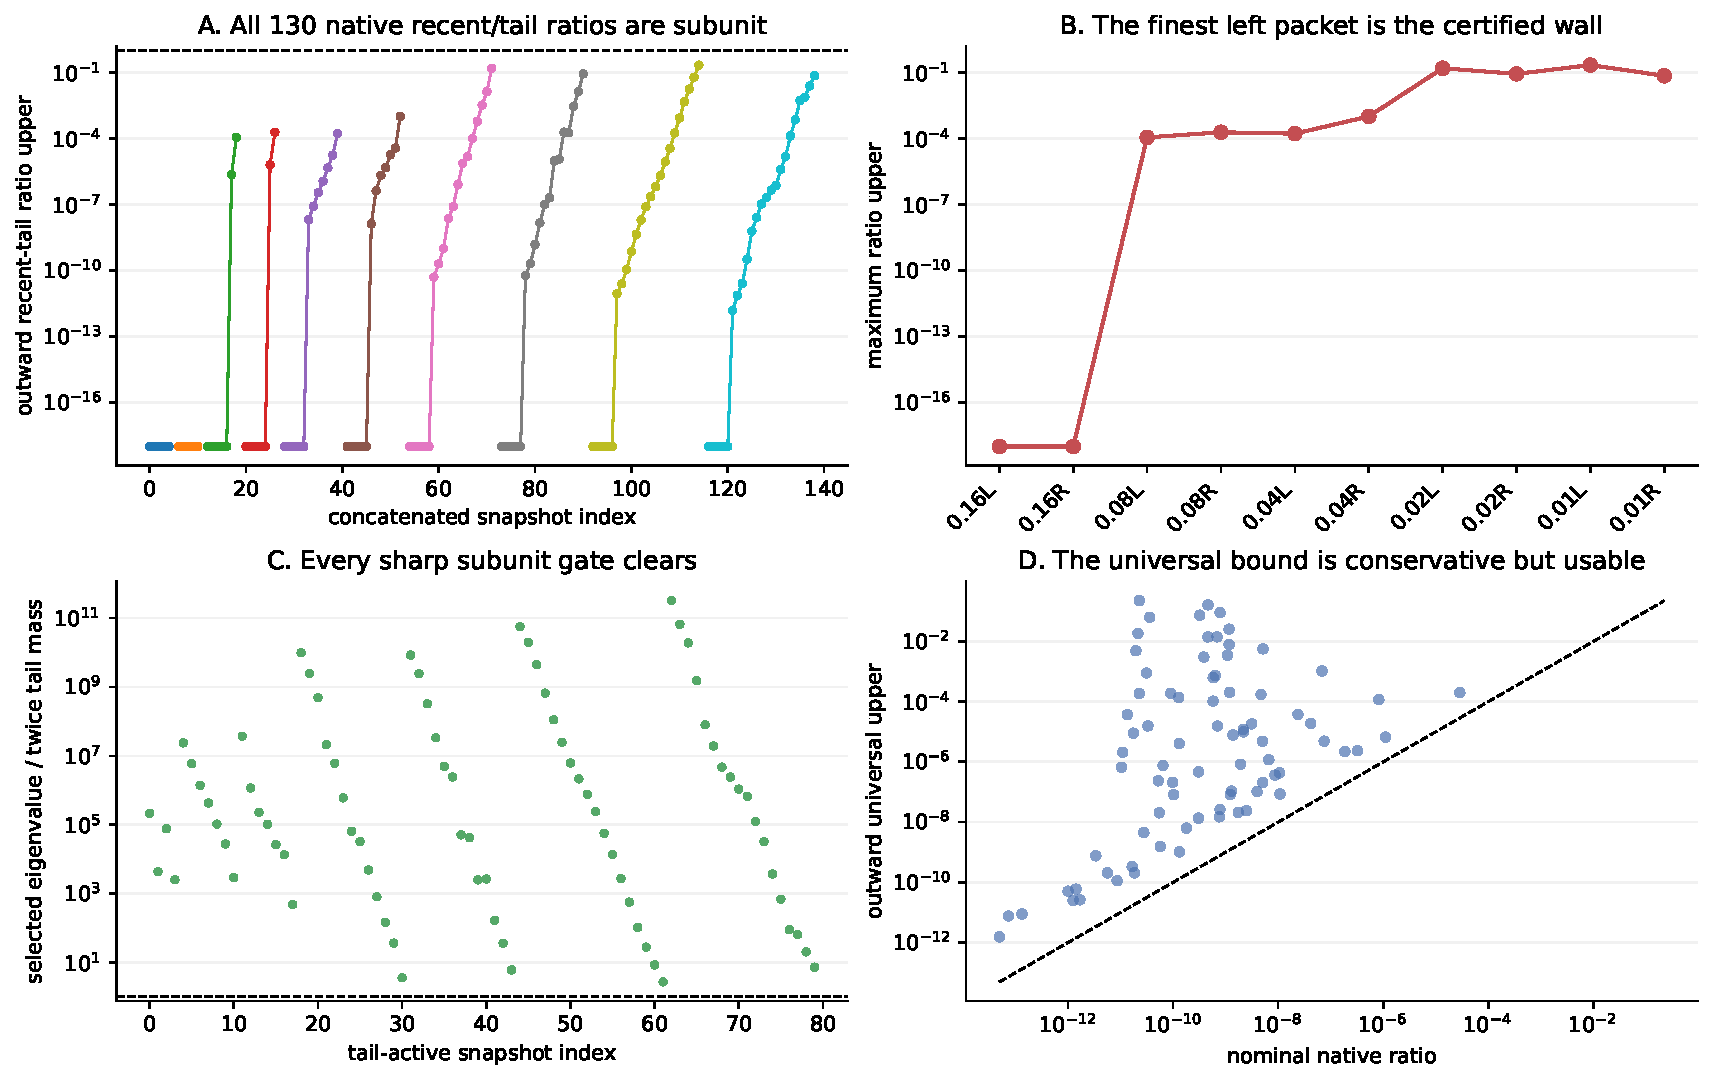
\includegraphics[width=\textwidth]{figures/native_spectral_reset_memory_pair.pdf}
\caption{Subunit native memory-pair bounds, channel maxima, sharp gate
margins, and comparison with direct nominal generalized ratios.}
\label{fig:audit}
\end{figure}

\section{Consequence and claim boundary}
RH-155 supplies the correlated object required by RH-153.  On any certified
snapshot, the native recent Gram is positive definite and the old tail is a
strictly subunit Loewner fraction of it.  Congruence transport preserves that
fraction exactly, so no inverse-overlap square is incurred.

The remaining conceptual interface is important: $G_t=U_t^*R_tU_t$ is a
native memory Gram, whereas RH-130--RH-148 used a recent projected-cross
action Gram and additional wedge/capacity factors.  We have not proved those
objects equivalent, supplied an all-level selected-eigenvalue lower, closed
Stage A, constructed a Hilbert--Polya operator, identified zeta zeros, or
proved the Riemann Hypothesis.

\bibliographystyle{plainnat}
\bibliography{references}
\end{document}
